\chapter{Dimensioning and Tolerancing}


    \section{Introduction}

        Currently available CAD data models are adequate in terms of providing
	a unique and unambiguous representation of the geometry of a part, but 
	these models
    only provide information about the nominal size of the part~\cite{Roy88}.
	They do not support or reason about dimensioning and tolerancing (D \& T)
	and other
    geometric inaccuracies. A new data representation scheme has been proposed 
	here, based on 
    feature-based principles which takes advantage of available product 
    data structures and adds dimensioning capability to them.

    A complete mapping of design features to manufacturing features has 
	been the goal of several recent and current research projects in the field 
	of feature-based design. The D \& T capability plays an important role 
    as it dictates how the part is to be made and to what specifications.

    Previously, designers would design the part in such a way as to 
    ensure proper functionality. The inclination was generally towards having 
	tighter dimensional control. Manufacturing demands looser 
	dimensional control because of the high cost of precision machining. 
	Resolving these
    conflicting viewpoints requires a system which will design the part and
    perform manufacturing evaluation simultaneously so as to achieve a 
	balanced solution.

    The main aim of our research at Kansas State University is to develop such
    an integrated system. D \& T has been developed to a 
	large extent for
    components with rotational geometry. The present work tries to 
	extend the dimensioning and tolerancing capability 
    to generalized orthohedral components with encapsulated geometries.


	\section{Background}


	When CAD systems first emerged, the D \& T 
	methods that they incorporated were mostly drawing-based and needed human 
	intervention for calculation, representation and interpretation. With 
	advances in feature based design, efforts have been made to automate some 
	parts of this process. 


    Computer aided analysis for D \& T was introduced by TOLTECH (TOLerance 
	TECHnology)~\cite{Bjork}, which addresses the problem of assigning 
	tolerances so as to achieve minimum cost of manufacturing. It can also 
	distribute tolerances and calculate the tolerance chains of an individual 
	part.
 
 
    Requicha~\cite{Requi85} attempted to relate several representational
	issues in D \& T in the CSG-based solid modeler, PADL-1. The object is 
	created step by step with dimensional attributes built in and a dimensioned 	drawing was produced using the attribute information.
 
        The major areas of interest in this field can be grouped into four 
	categories :

		\begin{enumerate}
		\item
        Representation of D \& T
		\item
        Synthesis and analysis of D \& T
		\item
        Control of tolerances at different phases of Manufacturing
		\item
        Implications of D \& T in downstream CAM activities
		\end{enumerate}
 
        The problem that is usually encountered in current CAD systems is a lack		of support in the dimensioning and tolerancing capability. 
		This is a serious deficiency because it implies that such systems 
		cannot support many design and production activities that require the 
		dimensioning and tolerancing information, e.g., fully automatic 
		manufacturing~\cite{Req83}.


    	Bing~\cite{Bing} proposed a new scheme which can represent 
		variational geometry classes as well as the relationships between them.
		This is similar to a solid model that uses the geometrical entities to 
		represent the nominal geometry and topological entities to represent 
		the relationships.
        The nominal geometry is decomposed into some basic geometric primitives.
		The primitive is said to be resolved when its shape is defined from its 
		locations. Bing has used GBBs (Geometric Building Blocks ) as the basic 
		entity to represent D \& T information. The GBBs used are :

			\begin{itemize}
			\item
            Plane 
			\item
			Line
			\item
			Point
			\item
			Feature of Size
			\item
			Curve 
			\item
			Surface
			\end{itemize}
			Nominal features and GBBs are different. For example, for the
			feature cylinder, the GBBs are given by :

			\begin{displaymath}
			GBB = \{ axis(Line) \& Radius(Feature of size) \}
			\end{displaymath}
 
    DOF (Degrees of Freedom) determines the number of independent parameters 
	required to constrain a GBB fully in space.
		\begin{itemize} 
		\item
        Translational DOF   = $ x,y,z.$
		\item
        Rotational DOF      = $\alpha,\beta,\gamma.$
		\end{itemize} 
 
    Tolerance classes are derived based on DOFs and GBBs. Combinations of DOFs 
	give new tolerance classes. Tolerance zones are created by applying the 
	transformation matrices to nominal geometries.First, an FD graph (Dimension 
	adjacency graph) is created. The user specifies the dimensions by picking 
	the datum and target planes.
    Then, the arcs are developed. The FD graph transforms into an FDT (D \& T 
	adjacency graph) graph by filling in tolerance components $ [(dx,dy,dz) $ 
	and $ (d\alpha,d\beta,d\gamma) ]$ 
	with corresponding tolerance values. Implicit dimensions (which can take 
	any value) and tolerances can be overwritten if more than one edge occurs at
	a node.
 
    Lin~\cite{Lin} proposed a data structure with the following 
	characteristics :
 
	\begin{enumerate}
	\item
    Faces are represented by nodes
	\item
    Relationship between faces is represented by arcs
	\item
    The node at the top is a root (datum) node
	\item
    All the nodes except the {\em root} have one and only one parent
	\item
    Any loops in the structure represent redundant dimensioning
	\end{enumerate}

	\section{Deficiencies in current D \& T data models} \label{dtdiff}

	There are some major deficiencies in the representation scheme for 
	{\em dimensioning and tolerancing} in currently available feature-based 
	design systems. This section reviews their shortcomings with a few 
	examples :


	\begin{itemize}

	\item
	\label{dtdiff1}

	It is a common practice in mechanical drawings to dimension co-planar 
	surfaces with a single (common) dimension (see Fig.~\ref{dtlak1})


       \begin{figure}[htbp]
            %\centerline{ \psfig{figure=DTLAK1.EPS,width=3.5in,height=5.0in}}
            \hspace{2cm}
            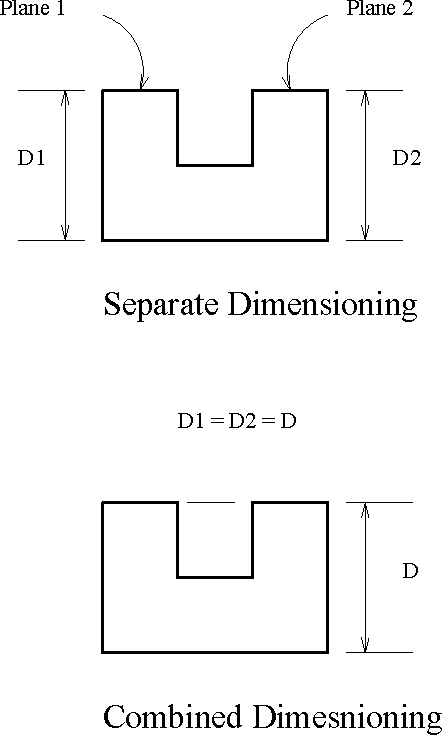
\includegraphics[width=3.5in,height=5.0in]{DTLAK1.pdf}
            \caption{Common dimensioning for co-planer surfaces}
            \label{dtlak1}
        \end{figure}


	Most of the current systems force the user to dimension plane 1 and plane 2 
	separately.
	In some cases, the user may want to dimension them separately, as he/she 
	would like to specify different tolerances on the dimensions. The data model
	should provide a mechanism to combine as well as separate the dimension
	primitives depending on the user request.

	\item
	\label{dtdiff2}

	There could be more than one way of dimensioning a part (see Fig 
	~\ref{dimcyl}). 
        \begin{figure}[htbp]
	%            \centerline{ \psfig{figure=dimcyl.ps,width=3.0in,height=5.5in}}
	            \hspace{2cm}
	            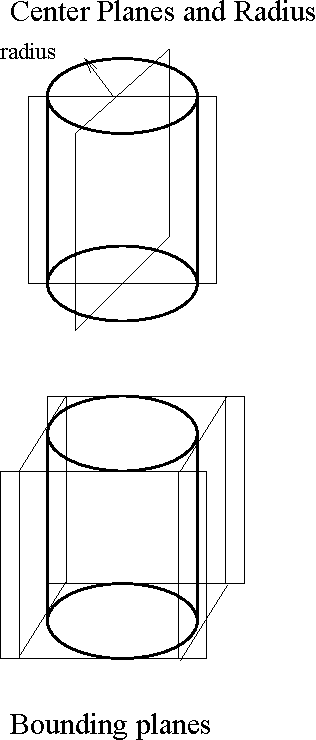
\includegraphics[width=3.0in,height=5.3in]{DIMCYL.pdf}
            \caption{Different dimensioning schemes for cylinder}
            \label{dimcyl}
        \end{figure}


	The dimensioning and tolerancing data model
    should have the capability to present all of them to the user and allow the
	user to make the choice. Most existing systems only allow one way to
	dimension a given feature.

	\item
	\label{dtdiff3}

	There is very little support for dimensioning free-form surfaces. 
	The present system provides the capability to dimension individual 
	surface points and also to group them with other dimensioning primitives 
	if necessary (see Fig. ~\ref{dimbsp}).



        \begin{figure}[htbp]
            %\centerline{\psfig{figure=dimbsp.ps,width=3.0in,height=5.0in}}
                        \hspace{2cm}
            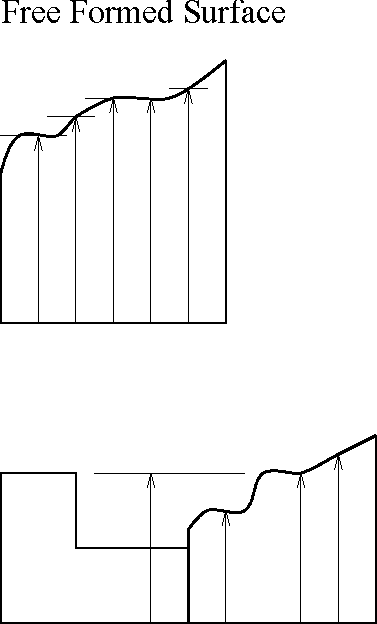
\includegraphics[width=3.0in,height=5.0in]{DIMBSP.pdf}

            \caption{Dimensioning scheme for B-spline}
            \label{dimbsp}
        \end{figure}

	\end{itemize}


	\section{Basic Concepts}

	The basic dimensioning primitives are :
		\begin{itemize}
		\item
		Dimension Planes
		\item
		Size dimensions
		\end{itemize}

	Most of the dimensioning is performed using dimensioning planes which are
	contributed
	by external as well as the internal shape. All dimensions are denoted
	as the distance between two dimension planes. Some dimensions
	like ``radius'' in the case of a cylinder are generally not modelled as 
	a distance
	between two planes. For such entities, a primitive called {\em size 
	dimension} is proposed. It is contributed by the internal shape.


	The dimensioning information for a feature can be decomposed into the
	following two categories
		\begin{enumerate}
		\item
		External or locational dimensions
		\item
		Internal or size dimensions
		\end{enumerate}

	For example, the dimensioning information of a cylinder can be decomposed as
	follows :
		\begin{itemize}
		\item
		{\em Locational} : top and bottom planes, and two mutually
		perpendicular middle planes along the axis
		\item
		{\em Size} : radius of the cylinder
		\end{itemize}
	The idea of {\em external shape} and {\em internal shape} explained
	earlier matches this concept very well, as the locational dimensions are
	defined with respect to the external shape while the size dimensions
	are defined by the internal shape.

	The external shape of each feature contributes dimensioning planes which 
	fix its position in the global coordinate system.
	The internal shape contributes planes and / or parameters (which are 
	specific to the 
	internal geometry) to fix the internal shape with respect to the external 
	shape.

	\section{Dimensioning and Tolerancing model}

		\subsection{Graph Representation}
		
		A graph data structure is used to model dimensioning and tolerancing
		information. A graph contains nodes interconnected by arcs. The nodes
		in the D \& T graph model represent one or more 
		{\em dimensioning primitives} while arcs represent dimensioning and
		tolerancing information. Various operations required in the context of
		dimensioning and tolerancing can be effectively formulated in terms
		of graph algorithms For example, the detection of over-dimensioning
		corresponds to the detection of cycles in the graph.

		\subsection{The D \& T Graph Model}

        The D \& T model proposed here takes advantage of external
        encapsulation and internal shape geometry. 
        Two graphs are used to represent the D \& T information for the 
		component :

		\begin{enumerate}
			\item
            Reference Dimension Graph (RDG)
			\item
            Specified Dimension Graph (SDG)

		\end{enumerate}

		The RDG is a relatively static data model and consists of a tree for
		each direction that has at least one plane normal to it. The tree is 
		of depth one and has a single root.
		The normal directions are grouped into X, Y, Z, and ``other''. The
		root in each set acts as a datum plane with respect to which all the
		other planes (represented by leaf nodes in the same tree) are
		dimensioned. The RDG forms a base with the help of which dimensions
		between any two planes can be computed.

		The SDG is a graph with the same nodes as the RDG, but its topology 
		is specified by the user (see Fig. ~\ref{rdgsdg}). The user never
		has to input the dimension while changing the SDG, those are
		computed internally with the help of the RDG.

        \begin{figure}[htbp]
            %\centerline{\psfig{figure=rdgsdg.ps,width=3.0in,height=5.0in}}
                                    \hspace{2cm}
            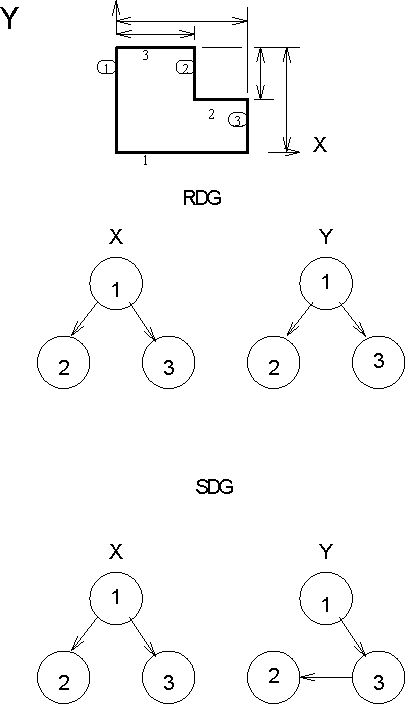
\includegraphics[width=3.0in,height=5.0in]{RDGSDG.pdf}

            \caption{The RDG and the SDG}
            \label{rdgsdg}
        \end{figure}
     \begin{figure}[htbp]
            %\centerline{\psfig{figure=dimgra.eps,width=3.0in,height=5.0in}}
                                    \hspace{2cm}
            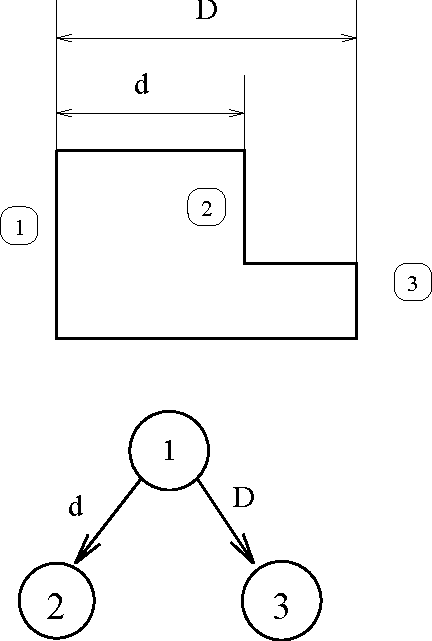
\includegraphics[width=3.0in,height=5.0in]{DIMGRA.pdf}
            \caption{Dimension Graph}
            \label{dimgra}
        \end{figure}

        The RDG and the SDG are created by default at the start 
		(see Fig. ~\ref{dimgra})
		and are initially identical. The RDG remains unchanged in structure
        for the component as long as the component's topology is unchanged. 
		It is hidden from the user, while the SDG is the one
        on which the user operates. The graph topology of the SDG may be 
		changed by the user to suit the needs of the dimensioning scheme.
		All changes to the SDG are validated internally with
        the help of the RDG. Any changes to the block structure of the
		component such as the addition of a new block, will 
		change both the RDG and the SDG. Geometric editing changes do not 
		change the topology of these graphs but change the values of the 
		dimensions stored in the dimension arcs.

		There are separate RDGs and SDGs for each direction. The directions
		are X, Y, Z, and ``Other''. The ``Other'' direction set consists of all
		the directions which are not coordinate directions.
		is further sorted according to the value of the normal so
		that all the planes having the same normal will form one RDG and one 
		SDG.

   


        \subsection{Data Structures}

			\begin{enumerate}
			\item
            A dimension graph contains a list of dimensioning Nodes.
			\item
            A dimensioning node contains information about the dimensioning
            primitive which it represents and also a list of dimensioning arcs
            going out from it.
			\item
            A dimensioning primitive is the actual dimensioning entity stored
			in the dimensioning node.
			\item
            A dimensioning arc connects two dimensioning nodes with a 
			directional property, i.e. the source represents the reference 
			primitive and the
            destination represents the target to which the dimension has been
            specified. Each arc stores information about dimension and tolerance
            values. Arcs in the RDG store reference dimension/ tolerance values
            while arcs in the SDG store user-specified dimension and tolerance
            values.
			\item
			Each direction has a different RDG and 
			SDG. The dimension primitives are first sorted according to the
			value of the normal and then contributed to the dimension graphs
			for that direction.

			\item
			Tolerances are associated with each arc in the SDG. The RDG does not
			contain any tolerances.
			\end{enumerate}

        \begin{figure}[htbp]
            %\centerline{\psfig{figure=dimdata.ps,width=3.0in,height=3.0in}}
            \hspace{2cm}
            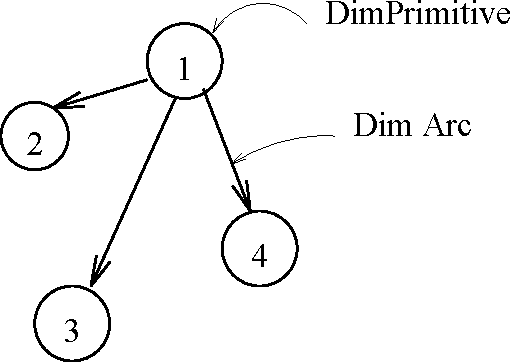
\includegraphics[scale=1.3]{DIMDATA.pdf}
            \caption{Graph Data Structure and Dimension Class}
            \label{dimdata}
        \end{figure}

		
        \subsection{Operations}

            \begin{enumerate}

            \item
            {\em Creation of the dimension graph }

                Depending on a block's internal shape, it contributes
                a preset number of dimensional primitives. Currently, only 
				planes
                have been used as dimensional primitives. Each primitive 
                gets mapped onto a dimensioning node and gets added to the
                dimension graph. While being added to the node list, the nodes
                are sorted according to axis and separate lists are
                maintained for each coordinate direction; planes that are not
				perpendicular to any coordinated axis are maintained in a
				fourth list. At the creation stage, the RDG and SDG have 
				the same 
				topological structure. In the RDG, the first dimension plane
				that is encountered acts as a datum dimension node and all the 
				other
				planes are dimensioned with respect to the first plane.
				The fourth category is further sorted according to the value
				to the normal of the planes. Each direction has its own RDG
				and SDG. Angles between two planes are represented by a
				dimensioning arc between dimensioning nodes of two different
				graphs. For example, if an angle needs to be specified between
				a plane in the X direction and a plane in the Y direction, 
				then an arc
				is set from the node representing the first dimension plane
				in dimension-graph-X to the node representing the 
				second plane in dimension-graph-Y.
				
				
                The arcs store the value of the distance/angle between two 
				primitives. For non-coordinate directions which have faces
				perpendicular to them, lists are maintained and processed in 
				the 
				same way as the coordinate axes lists. Initially, the SDG 
				follows a datum dimensioning scheme. Once the initial SDG is
				complete, the user is free to make changes in its topology
				by redefining the connectivity while preserving all the
				nodes.
				
				\item
                    {\em Specifying the dimension between two primitives} :

                    If the user wants to specify the dimensions between any two
                    primitives, the following is the general procedure :

                    \begin{enumerate}
                    \item
                    Select two primitives from the same block or different 
					blocks.
                    Currently, only planes that are parallel can be 
					chosen.
                    \item
                    Specify the dimension value and the tolerance.

                    \end{enumerate}

                    When this input is given, the two selected primitives are 
					located in the RDG and are checked for connectedness to
					ensure that a path exists between them. If no such path is
                    found, an error message is issued since the dimension 
					cannot be specified. If a path is found, the value of the
					dimension is computed by adding (or subtracting)
                    and is checked with the value specified by the
                    user. If this matches, checks are made to see if the
					modification will lead to over-dimensioning or under-
					dimensioning (see item 3 below). If this check is passed, 
					the SDG is modified while the RDG is kept unchanged.

				
        \begin{figure}[htbp]
            %\centerline{\psfig{figure=specdim.ps,width=2.0in,height=6.0in}}
            \hspace{4cm}
            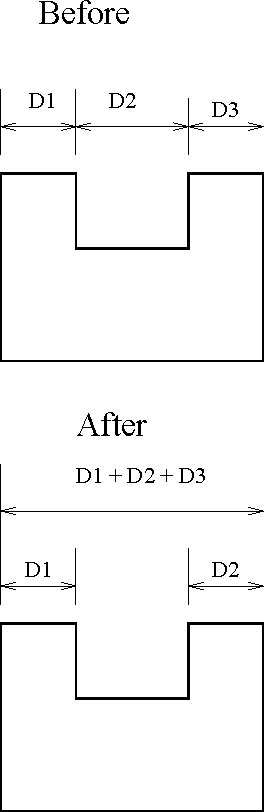
\includegraphics[scale=1.5]{SPECDIM.pdf}
            \caption{Specifying dimension between two planes}
            \label{specdim}
        \end{figure}


    \item
    {\em Change in Datum} :
    Datum, chain and mixed dimensioning are the three types of dimensioning 
	schemes normally followed in specifying dimensions. In datum

    dimensioning, one reference plane is chosen and all the
    other primitives are dimensioned with respect to that plane.
    In the manufacturing view, this datum feature is made first 
    and all the other features are manufactured or inspected with respect 
	to the datum.

    In chain dimensioning, the reference plane is the next plane along that 
	direction i.e. the destination primitive of the previous dimension becomes 
	the reference primitive of the next dimension.

    Mixed dimensioning contains more than one datum primitive from which the 
	rest of the primitives are dimensioned.

	The user may want to change the dimensioning scheme to any of the above
	mentioned dimensioning scheme. This is accomplished by changing to
	one or many datum planes in a single direction. The algorithm
	presented below describes the process of changing the datum plane for
	the case of datum dimensioning.

		\begin{itemize}
		\item
		The block list and the plane list are presented to the user for 
		selection of the datum plane.
		\item
		Each of the remaining nodes in the appropriate SDG is checked for a 
		path between
		itself and the new datum plane in the RDG. If found, an arc is set up
		between the new datum node and the second node under consideration.
		The dimension value is automatically computed by adding up the
		dimension values while traversing the path.

		\item
		The process is repeated until all the nodes in the SDG are checked.
		\end{itemize}

	        \begin{figure}[htbp]
	            %\centerline{\psfig{figure=chgdat.ps,width=4.0in,height=3.0in}}
	            \hspace{4cm}
	            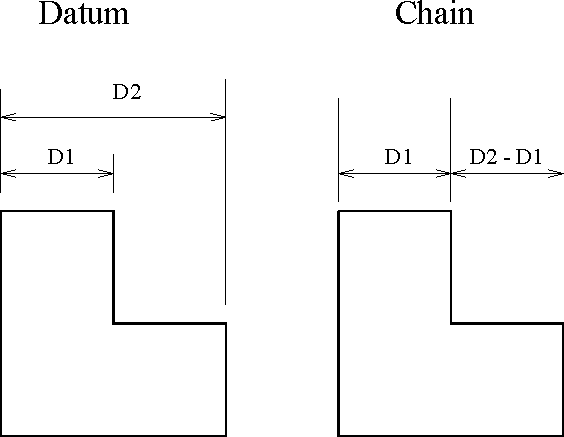
\includegraphics[scale=1.2]{CHGDAT.pdf}
	            \caption{Change of Datum Plane}
	            \label{chgdat}
	        \end{figure}

    \item
    {\em Detection of missing or redundant dimensions} :
        When a user specifies a new dimension, care is taken to verify that this
        does not introduce redundancy into the dimensioning scheme. This is
		easily accomplished, because a cycle in the graph means there is a
		redundancy (see Fig. ~\ref{ovrdim}). Conversely, if there is no cycle, 
		there is no 
		redundancy. The existence of cycles can be easily checked by a graph
		algorithm~\cite{Rein}. Similarly, if any dimensions are missing, the 
		graph becomes
		un-connected. This can also be easily detected using a suitable graph
		traversal algorithm such as a depth first search.

        \begin{figure}[htbp]
            %\centerline{\psfig{figure=ovrdim.ps,width=3.0in,height=6.0in}}
            	            \hspace{4cm}
            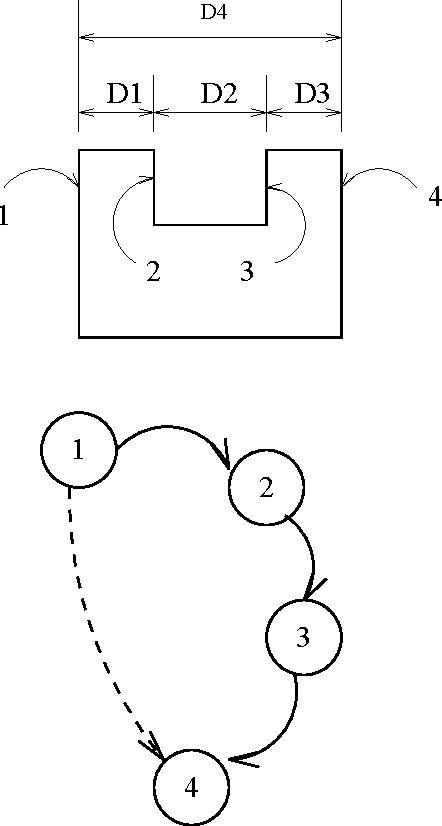
\includegraphics{OVRDIM.pdf}
            \caption{Over-dimensioning}
            \label{ovrdim}
        \end{figure}

    \item
    {\em Combination of primitives} :
    It has been common practice to dimension multiple coplanar faces 
    with a single dimension. This facility is provided in our scheme
	by allowing more than one dimensioning plane to be combined into
	a single dimensioning primitive, i.e., all these planes jointly
    behave as a single dimensioning primitive. If the user needs to
    separate out a plane for any reason (such as dimensioning different 
	tolerance values) the desired dimensioning planes can be delinked from the
    dimensioning primitive and a new dimensioning primitive corresponding to
	this plane can be created.

    \item
    {\em Query of Dimension} :
	If the user wants to query the distance between any two primitives, this 
	option
	can be used. The user must first specify the two blocks and the two plane
	primitives. A graph traversal algorithm first locates the two primitives
	in the SDG, 
	finds the unique path between them and computes the distance by summing
	the dimension attributes on the arcs that make up the path. Tolerance
	stacking is also determined in this way.
	\end{enumerate}

	\subsection{B-spline Dimensioning}
	\label{dimpts}

	Formation of the RDG and the SDG requires contribution of the dimensioning
	planes from individual blocks. These planes can be used to specify a 
	dimension with any other dimensioning plane. It is necessary that the
	B-spline surface provides not only the dimensioning planes corresponding 
	to the
	external rectangular block but also the dimensioning planes corresponding
	to selected points on the profile. 

		The dimensioning procedure is as follows :
            \begin{itemize}

            \item
            A two-dimensional view in the plane normal to the axis of the
				B-spline block is presented to the user. For example, if the
			axis of the B-spline is Z axis then the X-Y plane view is presented.

            \item
            For pre-specified intervals (say $n$), values $x_{1}$ to $x_{n}$
            are generated at equal intervals, where $x_{1}$ corresponds to the
			Xmin plane and $x_{n}$ corresponds to the Xmax plane.

            \item
            For each value of $x_{i}$ a corresponding $y_{i}$ is calculated
            from the profile equation.

            \item
            For each $i$, a plane normal to Y direction passing through $x_{i}$ 			and a plane normal to the X direction passing through $y_{i}$ are 
			contributed to the dimensioning procedure which is dealt with in 
			detail in section ~\ref{dimpts}.

	\item
	These dimensioning planes are contributed along with the side faces of the
	B-spline block.
	\item
	When the RDG and the default SDG are generated, all the planes are
	automatically included.

	\item
	The user is allowed to change the topology of the SDG as explained earlier.
	\end{itemize}

\section{Example of Basic Dimensioning}


		The example component is shown in Fig.~\ref{ex1comp} while Fig. ~\ref{ex1dim1} depicts how a component gets 
		dimensioned by default. Internally,
		the dimensioning scheme uses the graph data structures for reference
		dimension graph(RDG) and specified dimension graph(SDG) which are also 
		shown in the Fig.~\ref{ex1dim1}.
        \begin{figure}[htbp]
          %  \centerline{\psfig{figure=ex1dim1.ps,width=4.0in,height=5.0in}}
            \hspace{4cm}
            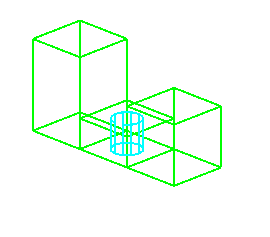
\includegraphics[scale=2.8]{EX1COMP.png}
            \caption{Example Component}
            \label{ex1comp}
        \end{figure}
  

		The Fig.~\ref{ex1dim1} shows default dimensioning scheme which is a
		datum dimensioning scheme along X axis.

       \begin{figure}[htbp]
          %  \centerline{\psfig{figure=ex1dim1.ps,width=4.0in,height=5.0in}}
                      \hspace{4cm}
            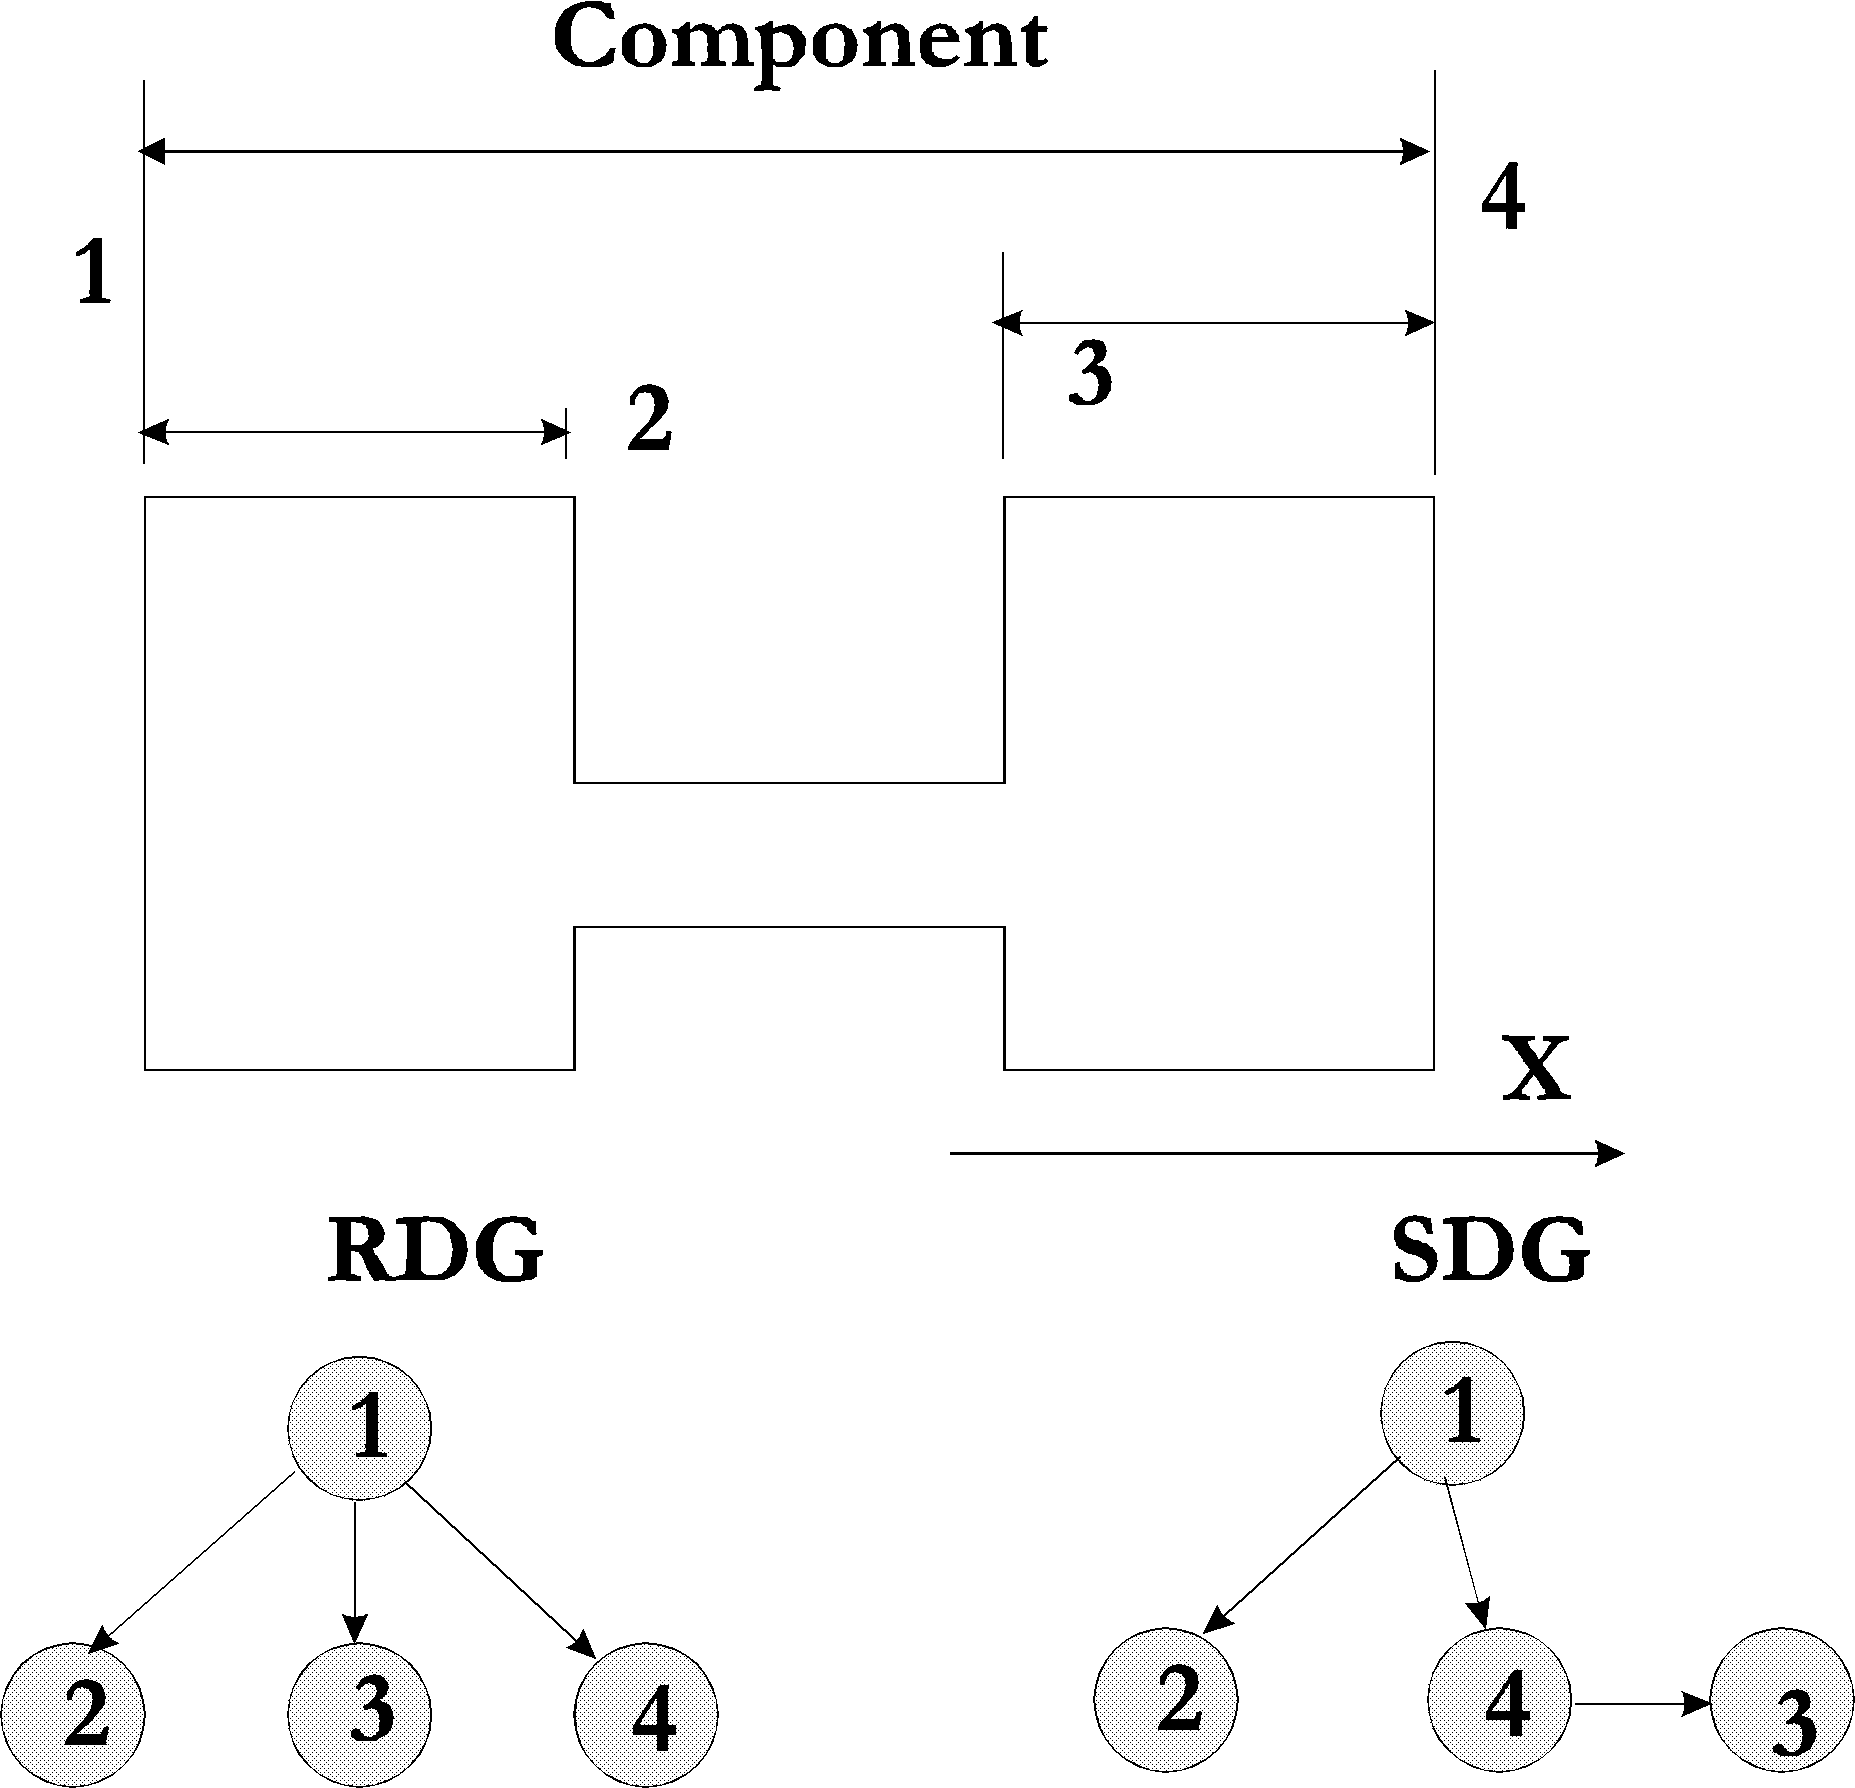
\includegraphics[scale=0.5]{SPEDIM.png}
            \caption{Dimensioning the component}
            \label{ex1dim1}
        \end{figure}
        
		Operations performed by the user to change the dimensioning scheme
		are reflected only in the specified dimension graph while the reference
		dimension graph remains unchanged. 
		The operations are listed below.
     
 
        
		\begin{enumerate}
		\item
					{\em Specifying the dimension between two planes} :

                    If the user wants to specify the dimension ``e'' between 
                    (say) plane 6 and plane 7, following actions are performed :
 
        
        \begin{figure}[htbp]
         %  \centerline{\psfig{figure=ex1dim2.ps,width=4.0in,height=5.0in}}
                               \hspace{4cm}
            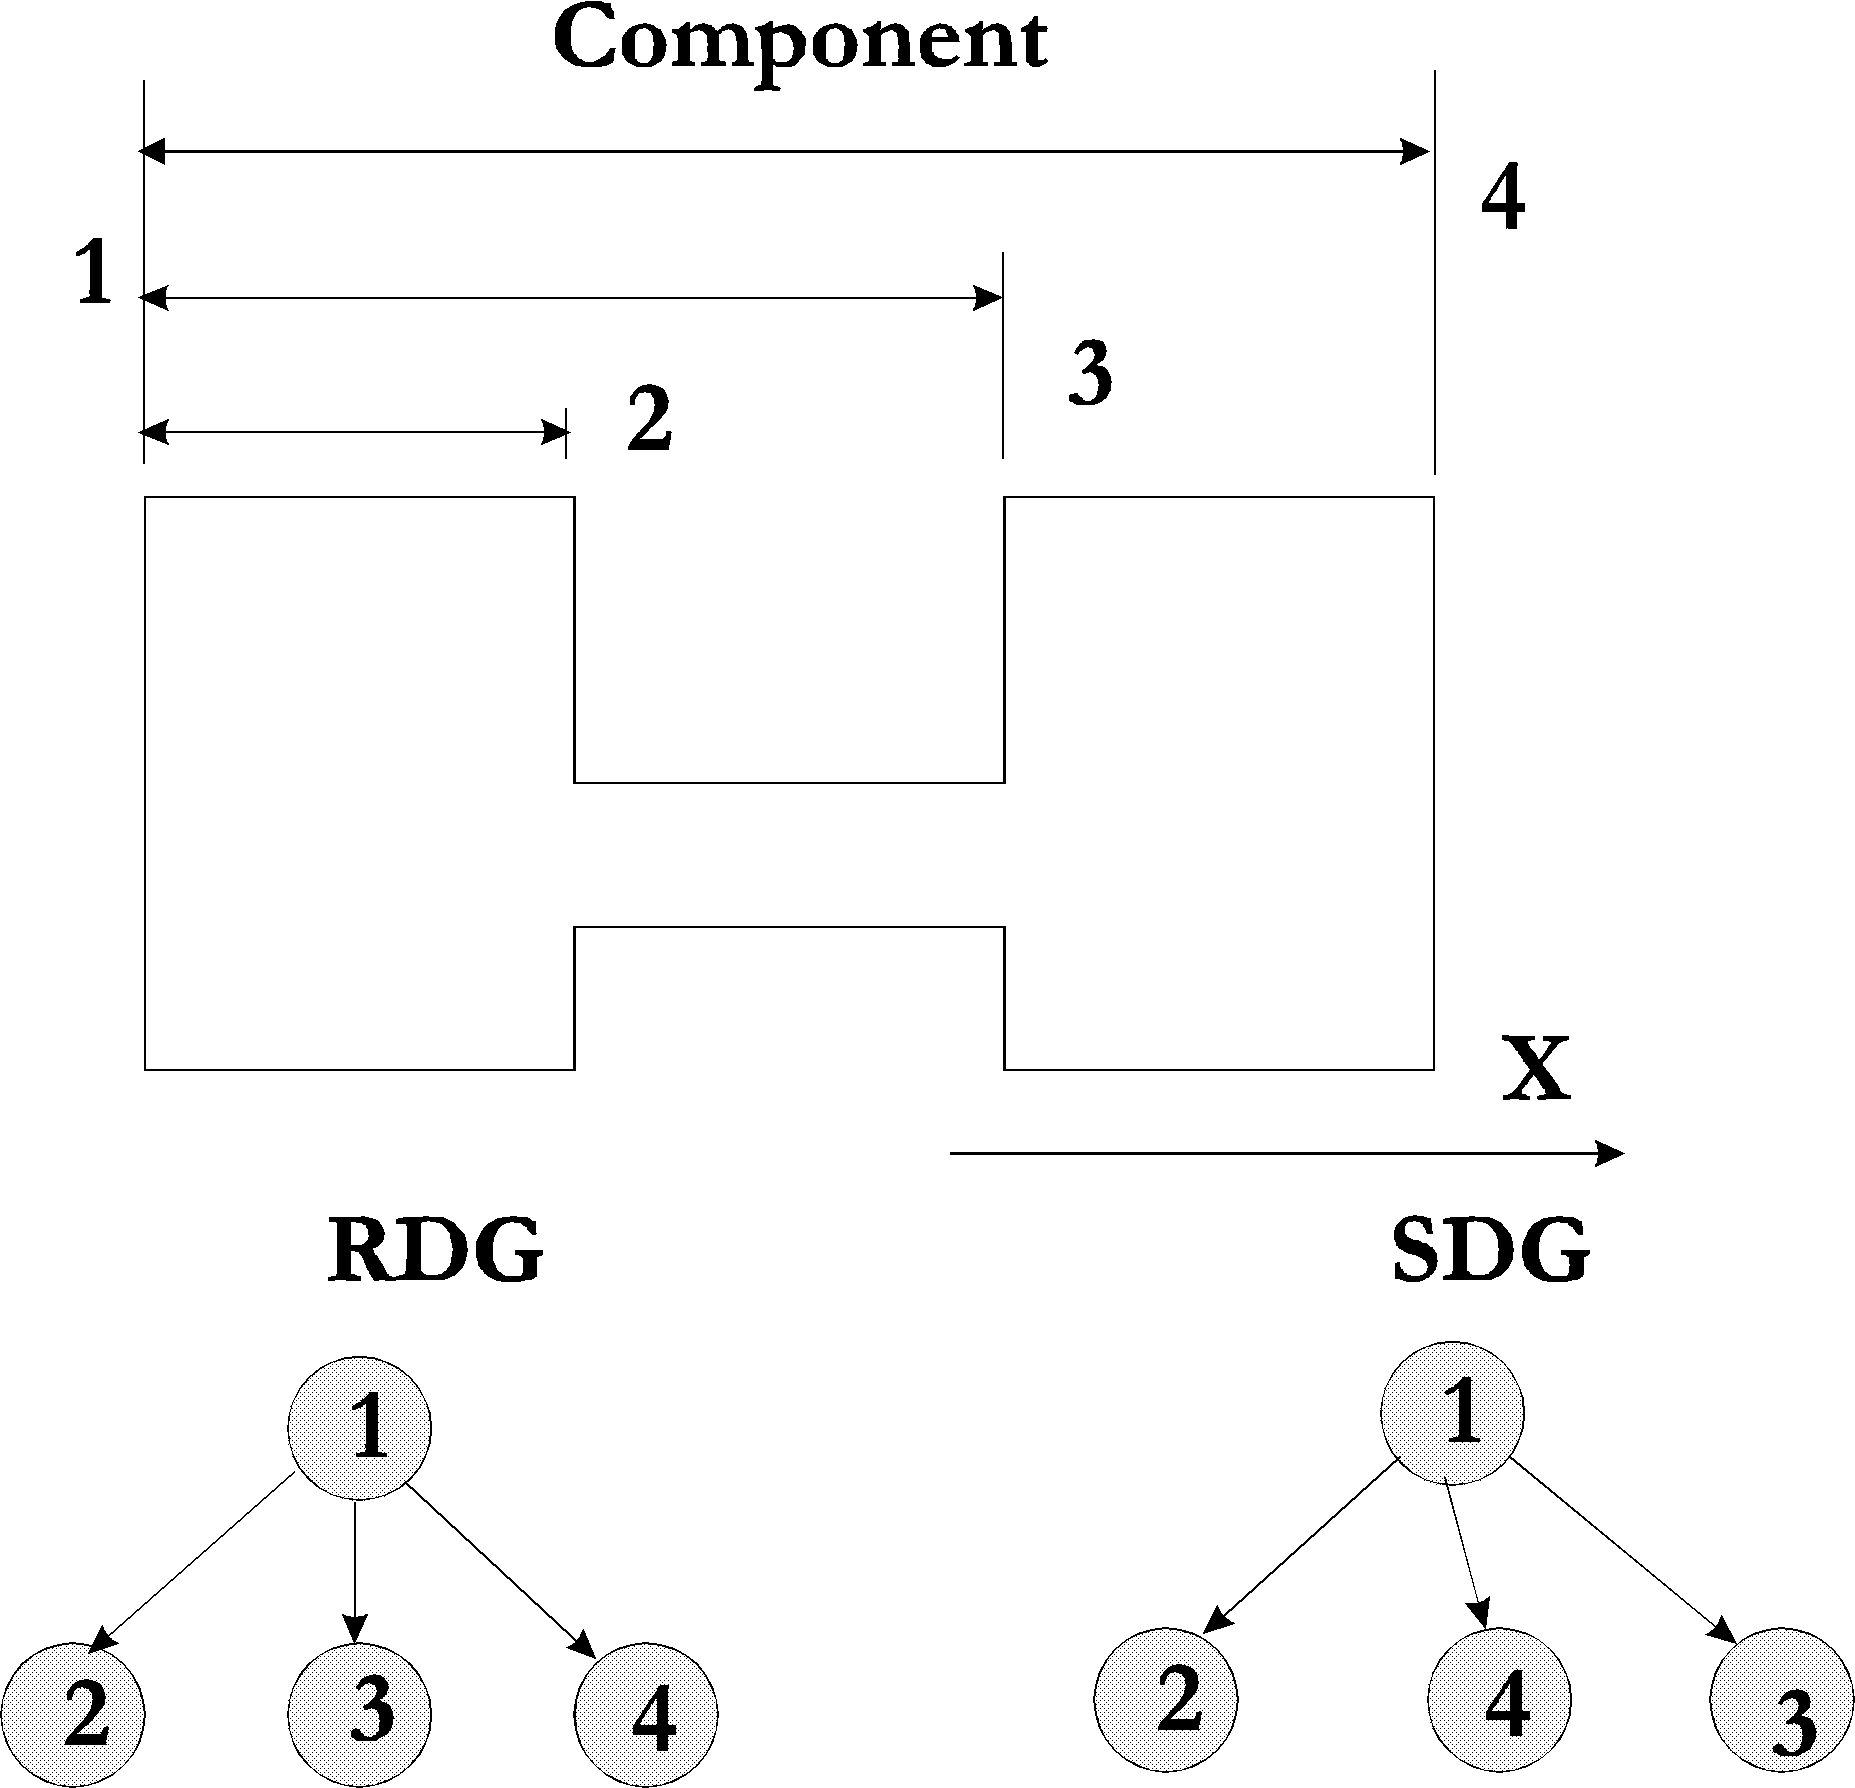
\includegraphics[scale=0.43]{DEFDIM.png}
            \caption{Specifying the dimension between two planes}
            \label{ex1dim2}
        \end{figure}


                    When the input is given, the two selected primitives are
                    located in the RDG and are checked for connectedness to
                    ensure that a path exists between them. If no such path is
                    found, an error message is issued since the dimension
                    cannot be specified. If a path is found, the value of the
                    dimension is computed by adding (or subtracting)
                    and is checked with the value specified by the
                    user. If this matches, checks are made to see if the
                    modification will lead redundancy in the 
                    dimensioning. If this check is passed,
                    the SDG is modified while the RDG is kept unchanged.
					The modified SDG is shown in Fig.~\ref{ex1dim2}, where
					a new arc is added between nodes 6 and 7 and the arc
					between nodes 1 and 7 is deleted as it would have created
					redundancy represented by a cycle.

		\item

    				{\em Change in Datum} :

    				The user may want to change the datum plane to plane 7
    				in the mentioned dimensioning scheme so that all the other
					planes are dimensioned with plane 7 as datum plane. 
					This is accomplished 
					by removing all arcs emanating from previous datum plane 1
					and making them emanate from the new datum plane 7 in
					the specified dimension graph.
					The modified SDG is shown in Fig~\ref{ex1dim3}.

        \begin{figure}[htbp]
         %   \centerline{\psfig{figure=ex1dim3.ps,width=4.0in,height=5.0in}}
                                        \hspace{4cm}
            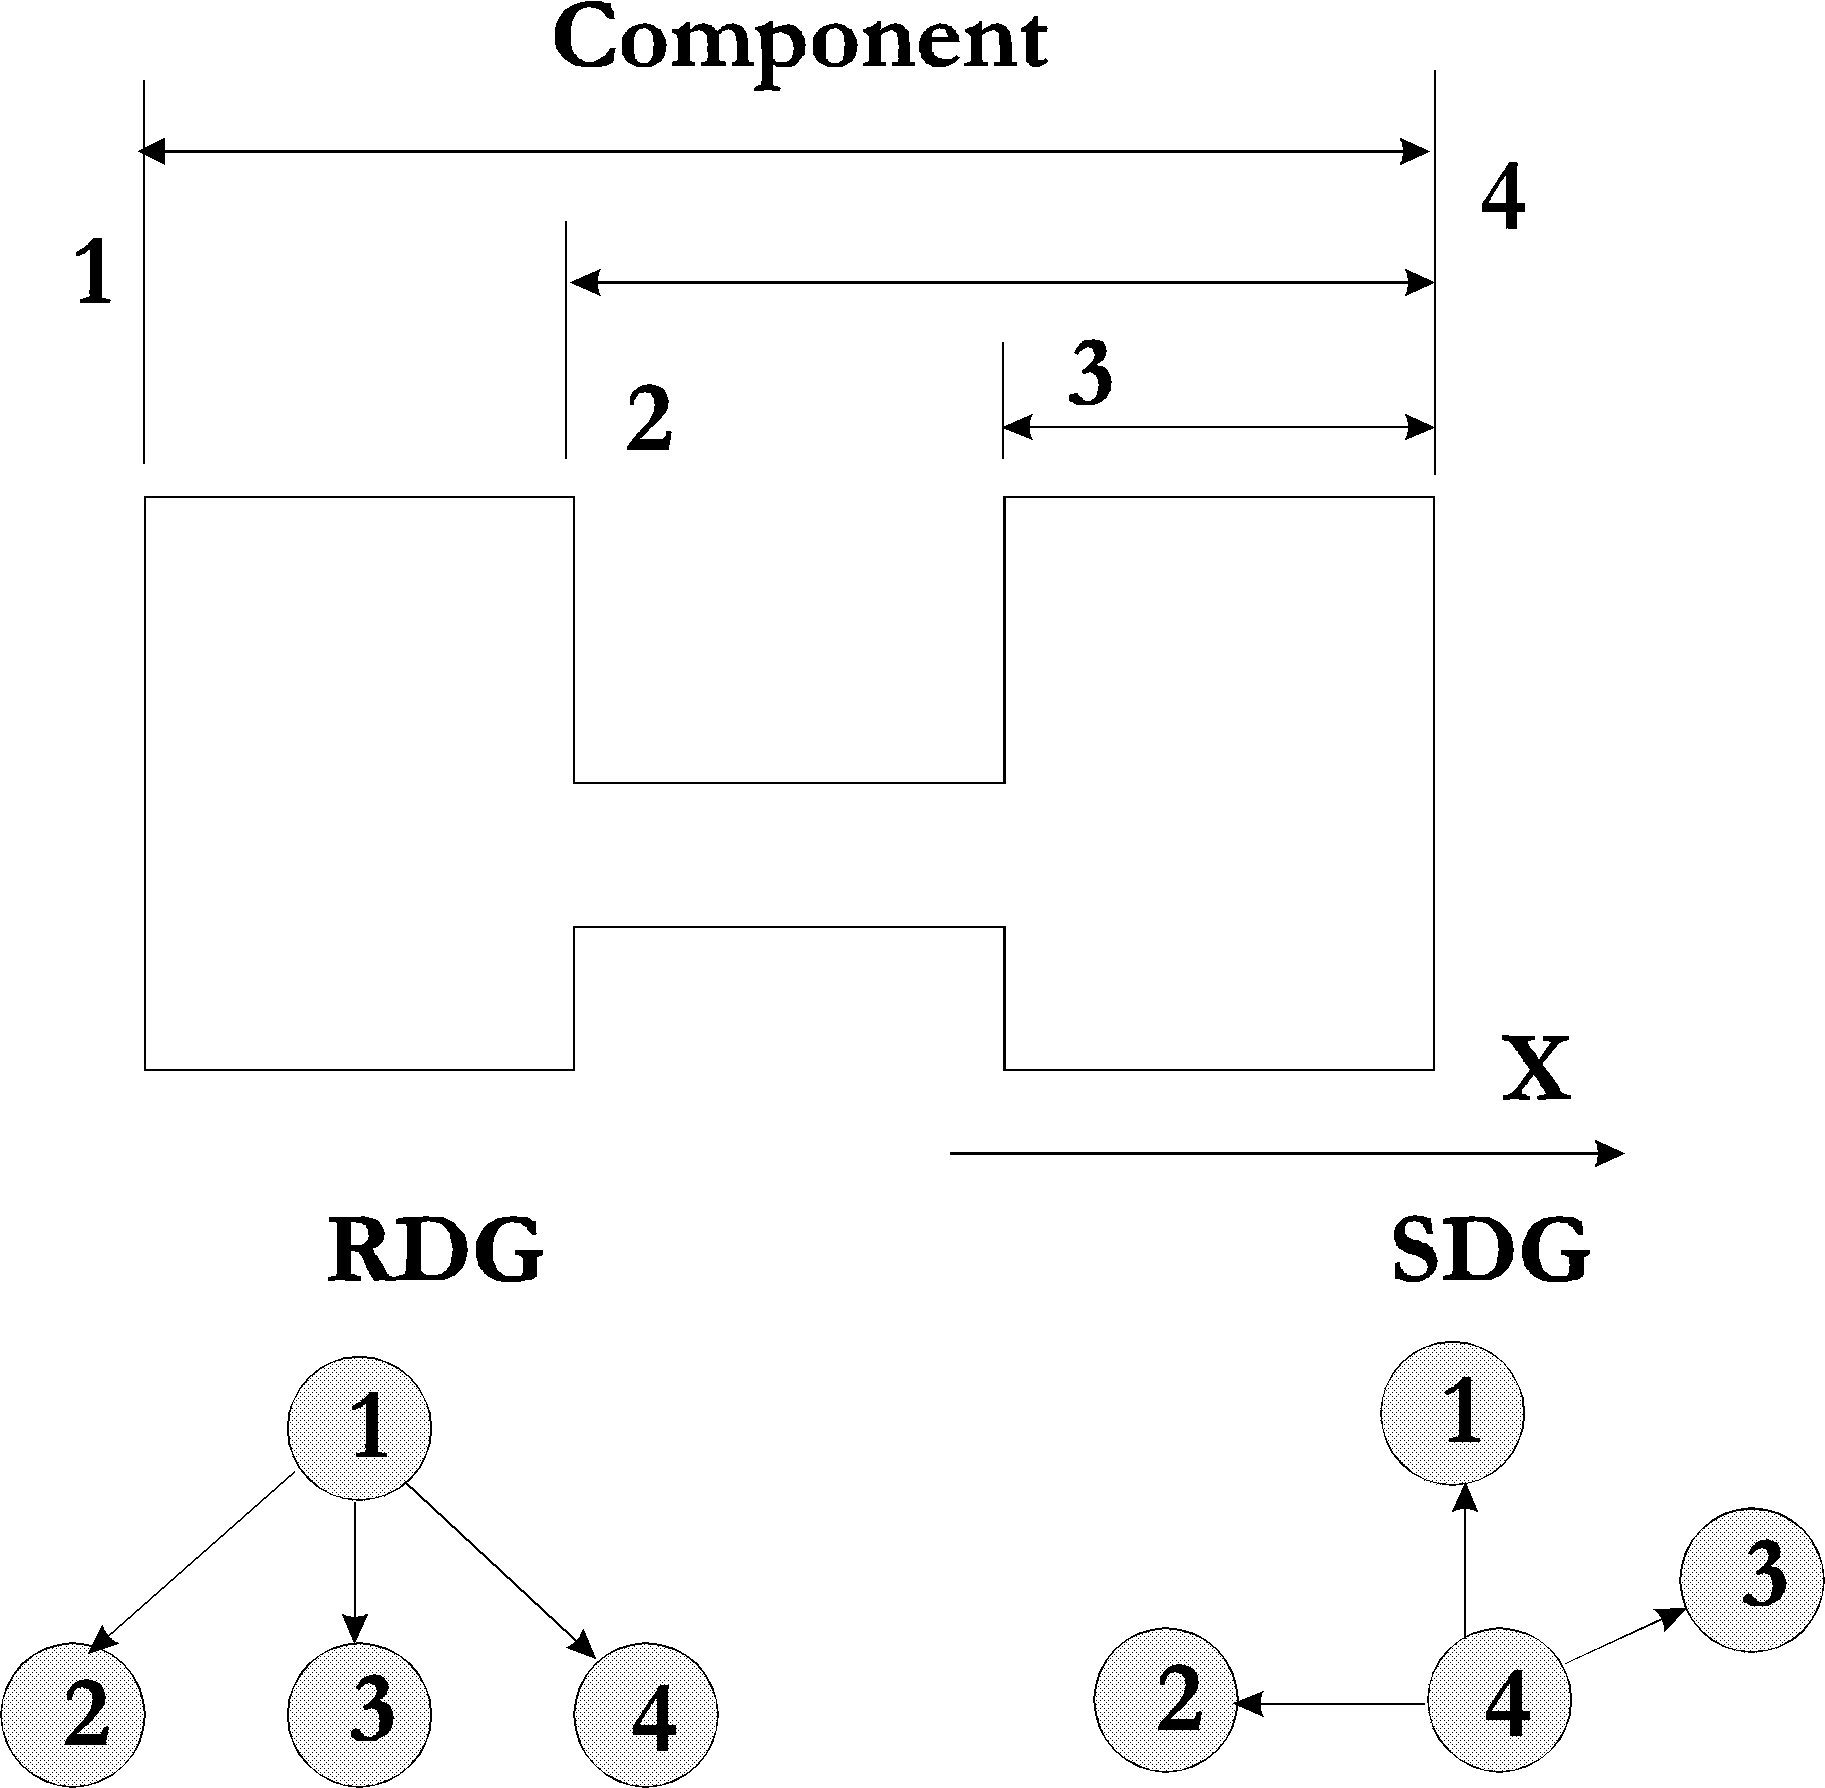
\includegraphics[scale=0.5]{CHGDAT.png}
            \caption{Change in Datum}
            \label{ex1dim3}
        \end{figure}

		\item

    				{\em Query of Dimension} :

    				If the user wants to query the distance between (say) 
					plane 2 and
					plane 7. A graph traversal algorithm first locates the 
					two primitives in the SDG, finds the unique path between 
					them and computes the distance by summing the dimension 
					attributes on the arcs that make up the path. 
					The computed distance is displayed to the user.

		\end{enumerate}

	\section{Bspline Dimensioning}

	The following example of a vice demonstrates the capability of 
	dimensioning the Bspline extruded block. The vice consists of two 
	rectangular blocks and a Bspline extruded block.
    Formation of the RDG and the SDG requires contribution of the dimensioning
    planes from individual blocks. These planes can be used to specify a
    dimension with any other dimensioning plane. It is necessary that the
    B-spline extruded block provides not only the dimensioning planes 
	corresponding to the
    external rectangular block but also the dimensioning planes corresponding
    to selected points on the profile of the Bspline.
    
           \begin{figure}[htbp]
          %  \centerline{\psfig{figure=ex1dim1.ps,width=4.0in,height=5.0in}}
            \hspace{4cm}
            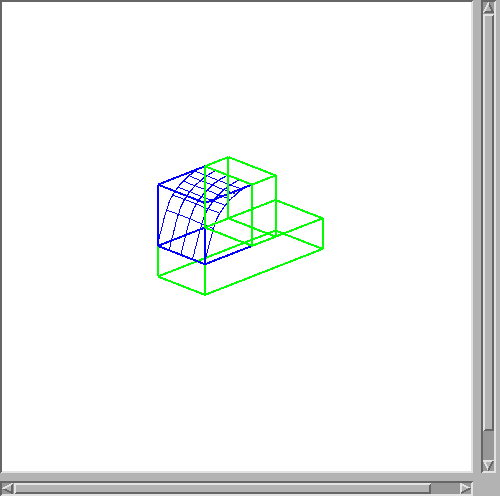
\includegraphics[scale=2]{EX2COMP.png}
            \caption{Example Component}
            \label{ex2comp}
        \end{figure}
        
	The example shows dimensions along X axis (see Fig.~\ref{ex2dim}).


        \begin{figure}[htbp]
          %  \centerline{\psfig{figure=ex2dim.ps,width=4.0in,height=5.0in}}
                  \hspace{4cm}
            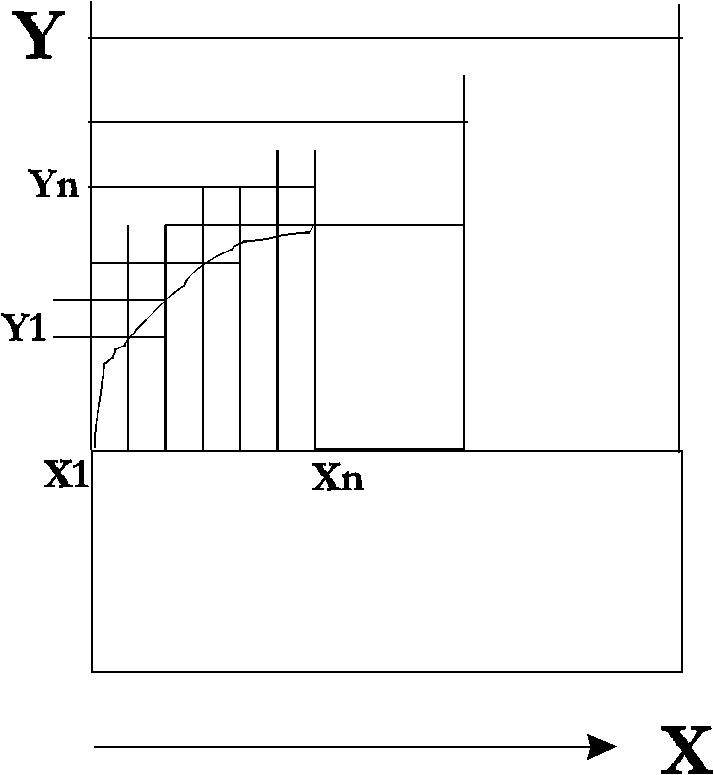
\includegraphics[scale=1]{BSPDIM.png}
            \caption{Bspline Dimensioning}
            \label{ex2dim}
        \end{figure}
        


        The dimensioning procedure is as follows :
            \begin{itemize}

            \item
            For pre-specified intervals (say $n$), values $x_{1}$ to $x_{n}$
            are generated at equal intervals, where $x_{1}$ corresponds to the
            Xmin plane and $x_{n}$ corresponds to the Xmax plane.
			Secant method is used to solve the non linear Bspline equation 
			to get the parameter value for each co-ordinate point $x_{i}$.

            \item
            For each parameter value corresponding to $x_{i}$ a corresponding 
			$y_{i}$ is calculated from the profile equation.

            \item
            For each $i$, a plane normal to Y direction passing through $x_{i}$
            and a plane normal to the X direction passing through $y_{i}$ are
            contributed to the dimensioning procedure.

			\item
			At the dimension graph level, these contributed planes are used
			dimension planes in the dimension scheme which is dealt with in
            detail in section ~\ref{dimpts}.
			\end{itemize}

